%!TEX program = xelatex

\documentclass[compress]{beamer}
%--------------------------------------------------------------------------
% Common packages
%--------------------------------------------------------------------------

\definecolor{links}{HTML}{663000}
\hypersetup{colorlinks,linkcolor=,urlcolor=links}

\usepackage[english]{babel}
\usepackage{pgfpages} % required for notes on second screen
\usepackage{graphicx}

\usepackage{multicol}

\usepackage{tabularx,ragged2e}
\usepackage{booktabs}

\setlength{\emergencystretch}{3em}  % prevent overfull lines
\providecommand{\tightlist}{%
  \setlength{\itemsep}{0pt}\setlength{\parskip}{0pt}}


\usetheme{hri}

% Display the navigation bullet even without subsections
\usepackage{remreset}% tiny package containing just the \@removefromreset command
\makeatletter
\@removefromreset{subsection}{section}
\makeatother
\setcounter{subsection}{1}


\newcommand{\source}[2]{{\tiny\it Source: \href{#1}{#2}}}

\usepackage{tikz}
\usetikzlibrary{mindmap,backgrounds,positioning,calc,patterns}
\usepackage{pgfplots}
\pgfplotsset{compat=newest}
\usepackage{circuitikz}

\graphicspath{{figs/}}

\title{ROCO222 \newline Intro to Sensors and Actuators}
\subtitle{Part 3 -- Electromagnetism}

\date{}
\author{Séverin Lemaignan}
\institute{Centre for Neural Systems and Robotics\\{\bf Plymouth University}}

\begin{document}

\licenseframe{github.com/severin-lemaignan/module-mobile-and-humanoid-robots}

\maketitle

\section{Electromagnetism}

{\fullbackground[scale=0.9,page=2]{ian-electromagnetism.pdf}
    \begin{frame}{Lines of field from a bar magnet}
    \end{frame}
}
{\fullbackground[scale=0.9,page=3]{ian-electromagnetism.pdf}
    \begin{frame}{Like poles repel and unlike poles attract}
    \end{frame}
}

{\fullbackground[scale=0.9,page=4]{ian-electromagnetism.pdf}
    \begin{frame}{Like poles repel and unlike poles attract}
    \end{frame}
}

{\fullbackground[scale=0.9,page=5]{ian-electromagnetism.pdf}
    \begin{frame}{Solenoid and bar magnets have similar lines of field}
    \end{frame}
}

{\fullbackground[scale=0.9,page=6]{ian-electromagnetism.pdf}
    \begin{frame}{Solenoid and bar magnets have similar lines of field}
    \end{frame}
}

{\fullbackground[scale=0.9,page=7]{ian-electromagnetism.pdf}
    \begin{frame}{Solenoid and bar magnets have similar lines of field}
    \end{frame}
}

{\fullbackground[scale=0.9,page=8]{ian-electromagnetism.pdf}
    \begin{frame}{Direction of conventional current}
    \end{frame}
}

{\fullbackground[scale=0.9,page=9]{ian-electromagnetism.pdf}
    \begin{frame}{Magnetic field strength H and flux density B}
    \end{frame}
}

{\fullbackground[scale=0.9,page=10]{ian-electromagnetism.pdf}
    \begin{frame}{FIeld around a current carrying wire}
    \end{frame}
}

{\fullbackground[scale=0.9,page=11]{ian-electromagnetism.pdf}
    \begin{frame}{The direction of induced magnetic field}
    \end{frame}
}

{\fullbackground[scale=0.9,page=12]{ian-electromagnetism.pdf}
    \begin{frame}{The direction of induced magnetic field}
    \end{frame}
}

{\fullbackground[scale=0.9,page=13]{ian-electromagnetism.pdf}
    \begin{frame}{Iron filings can show field around wire}
    \end{frame}
}

{\fullbackground[scale=0.9,page=14]{ian-electromagnetism.pdf}
    \begin{frame}{Iron filings can show field around wire}
    \end{frame}
}

{\fullbackground[scale=0.9,page=15]{ian-electromagnetism.pdf}
    \begin{frame}{Flux of magnetic field}
    \end{frame}
}

{\fullbackground[scale=0.9,page=16]{ian-electromagnetism.pdf}
    \begin{frame}{Ampere's law}
    \end{frame}
}

{\fullbackground[scale=0.9,page=17]{ian-electromagnetism.pdf}
    \begin{frame}{Ampere's law}
    \end{frame}
}

{\fullbackground[scale=0.9,page=18]{ian-electromagnetism.pdf}
    \begin{frame}{Simple example of Ampere's law}
    \end{frame}
}

{\fullbackground[scale=0.9,page=19]{ian-electromagnetism.pdf}
    \begin{frame}{Simple example of Ampere's law}
    \end{frame}
}

{\fullbackground[scale=0.9,page=20]{ian-electromagnetism.pdf}
    \begin{frame}{Ampere's law for current in straight wire}
    \end{frame}
}

{\fullbackground[scale=0.9,page=21]{ian-electromagnetism.pdf}
    \begin{frame}{Magnetic field due to current flow in a solenoid coil}
    \end{frame}
}

{\fullbackground[scale=0.9,page=22]{ian-electromagnetism.pdf}
    \begin{frame}{Iron filings show field inside solenoid}
    \end{frame}
}

{\fullbackground[scale=0.9,page=23]{ian-electromagnetism.pdf}
    \begin{frame}{Solenoid field}
    \end{frame}
}

{\fullbackground[scale=0.9,page=24]{ian-electromagnetism.pdf}
    \begin{frame}{Solenoid field}
    \end{frame}
}



{\fullbackground[scale=0.9,page=25]{ian-electromagnetism.pdf}
    \begin{frame}{Electromagnet core material}
    \end{frame}
}

{\fullbackground[scale=0.9,page=26]{ian-electromagnetism.pdf}
    \begin{frame}{Electromagnet using a nail}
    \end{frame}
}

{\fullbackground[scale=0.9,page=27]{ian-electromagnetism.pdf}
    \begin{frame}{Toroid coil}
    \end{frame}
}

{\fullbackground[scale=0.9,page=28]{ian-electromagnetism.pdf}
    \begin{frame}{Iron filings show field inside toroid}
    \end{frame}
}

{\fullbackground[scale=0.9,page=29]{ian-electromagnetism.pdf}
    \begin{frame}{B inside toroid coil}
    \end{frame}
}

{\fullbackground[scale=0.9,page=30]{ian-electromagnetism.pdf}
    \begin{frame}{B outside toroid coil}
    \end{frame}
}

\section{Conductors in magnetic field}

{\fullbackground[scale=0.9,page=32]{ian-electromagnetism.pdf}
    \begin{frame}{Magnetic force on wire}
    \end{frame}
}

{\fullbackground[scale=0.9,page=33]{ian-electromagnetism.pdf}
    \begin{frame}{Magnetic force between two wires}
    \end{frame}
}

{\fullbackground[scale=0.9,page=34]{ian-electromagnetism.pdf}
    \begin{frame}{Magnetic force between two wires}
    \end{frame}
}

\begin{frame}{Electromagnetic induction}

  Moving a magnet in a coil induces current


    \begin{center}
        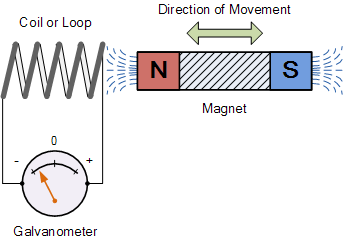
\includegraphics[width=0.6\linewidth]{part2/figs/image29}

    \scalebox{1.5}{Faraday's law of induction: $\displaystyle\mathcal{E} = -N \cdot \frac{d\Phi_B}{dt}$}

    \end{center}
\end{frame}

{\fullbackground[scale=0.9,page=36]{ian-electromagnetism.pdf}
    \begin{frame}{Faraday's law of induction}
    \end{frame}
}

{\fullbackground[scale=0.9,page=37]{ian-electromagnetism.pdf}
    \begin{frame}{Power used moving conduction in magnetic field B}
    \end{frame}
}

\section{Inductance}

{\fullbackground[scale=0.9,page=39]{ian-electromagnetism.pdf}
    \begin{frame}{Electrical resistance}
    \end{frame}
}

{\fullbackground[scale=0.9,page=40]{ian-electromagnetism.pdf}
    \begin{frame}{Electrical inductance}
    \end{frame}
}

{\fullbackground[scale=0.9,page=41]{ian-electromagnetism.pdf}
    \begin{frame}{Current in an LR circuit}
    \end{frame}
}

{\fullbackground[scale=0.9,page=42]{ian-electromagnetism.pdf}
    \begin{frame}{Current in an LR circuit}
    \end{frame}
}

{\fullbackground[scale=0.9,page=43]{ian-electromagnetism.pdf}
    \begin{frame}{Definition of inductance}
    \end{frame}
}

{\fullbackground[scale=0.9,page=44]{ian-electromagnetism.pdf}
    \begin{frame}{Inductance of a solenoid}
    \end{frame}
}

{\fullbackground[scale=0.9,page=45]{ian-electromagnetism.pdf}
    \begin{frame}{Inductance of a toroid}
    \end{frame}
}

{\fullbackground[scale=0.9,page=46]{ian-electromagnetism.pdf}
    \begin{frame}{Resistance of a coil}
    \end{frame}
}

{\fullbackground[scale=0.9,page=47]{ian-electromagnetism.pdf}
    \begin{frame}{Diameter of standard wire gauges (SWG)}
    \end{frame}
}

\section{Magnetic materials}

{\fullbackground[scale=0.9,page=49]{ian-electromagnetism.pdf}
    \begin{frame}{Types of magnetism: paramagnetism}
    \end{frame}
}

{\fullbackground[scale=0.9,page=50]{ian-electromagnetism.pdf}
    \begin{frame}{Types of magnetism: paramagnetism}
    \end{frame}
}

{\fullbackground[scale=0.9,page=51]{ian-electromagnetism.pdf}
    \begin{frame}{Types of magnetism: diamagnetism}
    \end{frame}
}

{\fullbackground[scale=0.9,page=52]{ian-electromagnetism.pdf}
    \begin{frame}{Types of magnetism: ferromagnetism}
    \end{frame}
}

{\fullbackground[scale=0.9,page=53]{ian-electromagnetism.pdf}
    \begin{frame}{Types of magnetism: ferromagnetism}
    \end{frame}
}

\section{Permanent magnets}

{\fullbackground[scale=0.9,page=55]{ian-electromagnetism.pdf}
    \begin{frame}{Permanent sources of magnetism}
    \end{frame}
}

{\fullbackground[scale=0.9,page=56]{ian-electromagnetism.pdf}
    \begin{frame}{Earth's magnetic field}
    \end{frame}
}

{\fullbackground[scale=0.9,page=57]{ian-electromagnetism.pdf}
    \begin{frame}{Ferrite magnets}
    \end{frame}
}

{\fullbackground[scale=0.9,page=58]{ian-electromagnetism.pdf}
    \begin{frame}{Alinico (AlNiCo)}
    \end{frame}
}

{\fullbackground[scale=0.9,page=59]{ian-electromagnetism.pdf}
    \begin{frame}{Samarium cobalt (SmCo)}
    \end{frame}
}

{\fullbackground[scale=0.9,page=60]{ian-electromagnetism.pdf}
    \begin{frame}{Neodymium magnets (NdFeB)}
    \end{frame}
}

{\fullbackground[scale=0.9,page=61]{ian-electromagnetism.pdf}
    \begin{frame}{Neodymium -- very powerful}
    \end{frame}
}

{\fullbackground[scale=0.9,page=62]{ian-electromagnetism.pdf}
    \begin{frame}{Magnetization or B-H curve of ferromagnetic material}
    \end{frame}
}

{\fullbackground[scale=0.9,page=63]{ian-electromagnetism.pdf}
    \begin{frame}{Magnetic hysteresis loop}
    \end{frame}
}

{\fullbackground[scale=0.9,page=64]{ian-electromagnetism.pdf}
    \begin{frame}{Important characteristic of permanent magnets}
    \end{frame}
}

{\fullbackground[scale=0.9,page=65]{ian-electromagnetism.pdf}
    \begin{frame}{Hard and soft magnetic materials}
    \end{frame}
}

{\fullbackground[scale=0.9,page=66]{ian-electromagnetism.pdf}
    \begin{frame}{Magnetic hysteresis loop for soft and hard materials}
    \end{frame}
}

{\fullbackground[scale=0.9,page=67]{ian-electromagnetism.pdf}
    \begin{frame}{Magnetic hysteresis loop for soft and hard materials}
    \end{frame}
}

{\fullbackground[scale=0.9,page=68]{ian-electromagnetism.pdf}
    \begin{frame}{Making a permanent magnet}
    \end{frame}
}


{\fullbackground[scale=0.9,page=69]{ian-electromagnetism.pdf}
    \begin{frame}{Demagnetizers}
    \end{frame}
}

\section{Magnetic circuits}

{\fullbackground[scale=0.9,page=02]{ian-magnetic-circuits.pdf}
    \begin{frame}{Magnetomotive force $\vec{F}$}
    \end{frame}
}

{\fullbackground[scale=0.9,page=03]{ian-magnetic-circuits.pdf}
    \begin{frame}{Electrical circuit analogy}
    \end{frame}
}

{\fullbackground[scale=0.9,page=04]{ian-magnetic-circuits.pdf}
    \begin{frame}{Magnetic circuit definitions}
    \end{frame}
}

{\fullbackground[scale=0.9,page=05]{ian-magnetic-circuits.pdf}
    \begin{frame}{Magnetic circuit definitions}
    \end{frame}
}

{\fullbackground[scale=0.9,page=06]{ian-magnetic-circuits.pdf}
    \begin{frame}{Reluctance of a magnetic path}
    \end{frame}
}

{\fullbackground[scale=0.9,page=07]{ian-magnetic-circuits.pdf}
    \begin{frame}{Magnetic circuit}
    \end{frame}
}

{\fullbackground[scale=0.9,page=08]{ian-magnetic-circuits.pdf}
    \begin{frame}{Analogy: electric \& magnetic circuits}
    \end{frame}
}

{\fullbackground[scale=0.9,page=09]{ian-magnetic-circuits.pdf}
    \begin{frame}{Reluctances combine like resistances}
    \end{frame}
}

{\fullbackground[scale=0.9,page=10]{ian-magnetic-circuits.pdf}
    \begin{frame}{Magnetic circuit with air gap}
    \end{frame}
}

{\fullbackground[scale=0.9,page=11]{ian-magnetic-circuits.pdf}
    \begin{frame}{Magnetomotive force: example 1}
    \end{frame}
}

{\fullbackground[scale=0.9,page=12]{ian-magnetic-circuits.pdf}
    \begin{frame}{Magnetomotive force: example 2}
    \end{frame}
}

{\fullbackground[scale=0.9,page=13]{ian-magnetic-circuits.pdf}
    \begin{frame}{Magnetic circuit for toroid}
    \end{frame}
}

{\fullbackground[scale=0.9,page=14]{ian-magnetic-circuits.pdf}
    \begin{frame}{Accounting for fringing}
    \end{frame}
}

{\fullbackground[scale=0.9,page=15]{ian-magnetic-circuits.pdf}
    \begin{frame}{Magnetic circuit with an air gap}
    \end{frame}
}

{\fullbackground[scale=0.9,page=16]{ian-magnetic-circuits.pdf}
    \begin{frame}{Magnetic circuit with an air gap}
    \end{frame}
}

{\fullbackground[scale=0.9,page=17]{ian-magnetic-circuits.pdf}
    \begin{frame}{Magnetic circuit with an air gap: numeric example}
    \end{frame}
}

{\fullbackground[scale=0.9,page=18]{ian-magnetic-circuits.pdf}
    \begin{frame}{Magnetic circuit with an air gap: numeric example}
    \end{frame}
}

{\fullbackground[scale=0.9,page=19]{ian-magnetic-circuits.pdf}
    \begin{frame}{Magnetic circuit with an air gap: numeric example}
    \end{frame}
}

{\fullbackground[scale=0.9,page=20]{ian-magnetic-circuits.pdf}
    \begin{frame}{Horseshoe magnetic circuit}
    \end{frame}
}

{\fullbackground[scale=0.9,page=21]{ian-magnetic-circuits.pdf}
    \begin{frame}{Parallel magnetic circuit and electrical analogy}
    \end{frame}
}

{\fullbackground[scale=0.9,page=22]{ian-magnetic-circuits.pdf}
    \begin{frame}{Parallel and series reluctances in magnetic circuits}
    \end{frame}
}

\section{Magnetic force}

{\fullbackground[scale=0.9,page=24]{ian-magnetic-circuits.pdf}
    \begin{frame}{Electromagnets can generate force}
    \end{frame}
}

{\fullbackground[scale=0.9,page=25]{ian-magnetic-circuits.pdf}
    \begin{frame}{Force: Derivative of energy with respect to distance}
    \end{frame}
}

{\fullbackground[scale=0.9,page=26]{ian-magnetic-circuits.pdf}
    \begin{frame}{Remember: inductance of a solenoid}
    \end{frame}
}

{\fullbackground[scale=0.9,page=27]{ian-magnetic-circuits.pdf}
    \begin{frame}{Energy in a magnetic field}
    \end{frame}
}

{\fullbackground[scale=0.9,page=28]{ian-magnetic-circuits.pdf}
    \begin{frame}{Relay closing current}
    \end{frame}
}

{\fullbackground[scale=0.9,page=29]{ian-magnetic-circuits.pdf}
    \begin{frame}{Relay closing current}
    \end{frame}
}

{\fullbackground[scale=0.9,page=30]{ian-magnetic-circuits.pdf}
    \begin{frame}{Relay closing current: example}
    \end{frame}
}

{\fullbackground[scale=0.9,page=31]{ian-magnetic-circuits.pdf}
    \begin{frame}{Horseshoe static magnetic force}
    \end{frame}
}

{\fullbackground[scale=0.9,page=32]{ian-magnetic-circuits.pdf}
    \begin{frame}{Solenoid motor}
    \end{frame}
}


\begin{frame}{}
    \begin{center}
        \Large
        That's all, folks!\\[2em]
        \normalsize
        Questions:\\
        Portland Square B316 or \url{severin.lemaignan@plymouth.ac.uk} \\[1em]

        Slides:\\
        \href{https://github.com/severin-lemaignan/module-mobile-and-humanoid-robots}{\small
        github.com/severin-lemaignan/module-introduction-sensors-actuators}


    \end{center}
\end{frame}



\end{document}
